\begin{figure}[htbp]
  \centering
  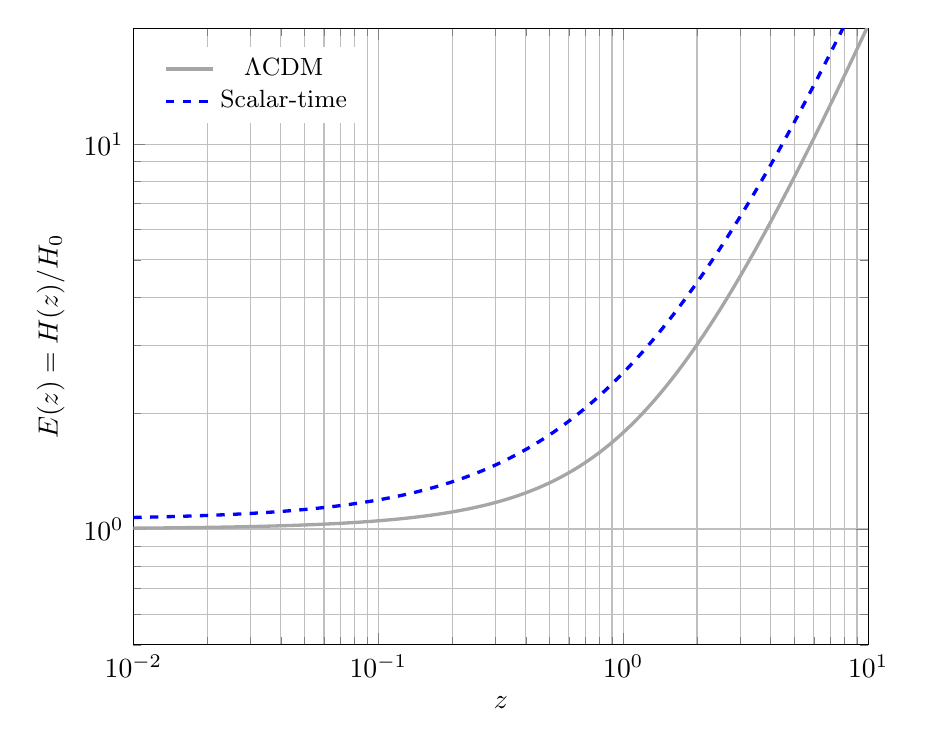
\begin{tikzpicture}
  \begin{axis}[
      width=0.9\textwidth,
      xlabel={$z$},
      ylabel={$E(z)=H(z)/H_0$},
      xmode=log, ymode=log,
      xmin=0.01, xmax=10,
      ymin=0.5,  ymax=20,
      grid=both,
      legend pos=north west,
      legend style={draw=none, font=\small}]
    % --- ΛCDM fiducial  ----------------------------------------
    \addplot[gray!70,very thick,domain=0.01:10,samples=220]
      {sqrt(4.2e-5*(1+x)^4 + 0.31*(1+x)^3 + 0.69)};
    \addlegendentry{$\Lambda$CDM}
    % --- Scalar-time model  ------------------------------------
    \addplot[blue,dashed,very thick,domain=0.01:10,samples=220]
      {sqrt(4.2e-5*(1+x)^4 + 0.50*(1+x)^3 + 0.62*(1+x)^2)};
    \addlegendentry{Scalar-time}
  \end{axis}
  \end{tikzpicture}
  %-------------------------------------------------------------
  \caption{Effective expansion history $E(z)$ for the scalar-time best-fit parameters (blue dashed) compared with a fiducial $\Lambda$CDM model (solid grey).  The two histories diverge only at $z\!\lesssim\!3$, making late-time probes (BAO, SNe, red-shift drift) the key discriminants.}
  \label{fig:EzCurve}
\end{figure}
